\documentclass[10pt]{article}
\usepackage[margin=1in]{geometry}
\usepackage{amsmath,amssymb}
\usepackage{graphicx}
\usepackage{booktabs}
\usepackage[colorlinks=true,linkcolor=blue,citecolor=blue,urlcolor=blue]{hyperref}
\usepackage{xcolor}

\title{\bf Thickness from Color by Inverting the Physics:\\ Self-Calibrating Differentiable Thin-Film Optics\\ for Region-Level 2D-Material Thickness Estimation}
\author{Benjamin Petrie\\ \small ORCID 0009-0005-5256-5382\\
\small Independent Researcher, Syracuse, New York, USA\\
\small \texttt{benpetriework@gmail.com}}
\date{}

\newcommand{\todo}[1]{\textcolor{red}{[TODO: #1]}}
\newcommand{\fillin}[1]{\textcolor{red}{\textbf{[#1]}}}  % numeric slots for \S5.10; must be empty at submission

\begin{document}
\maketitle

\begin{abstract}
Estimating the thickness of exfoliated two-dimensional flakes from ordinary optical micrographs is a foundational task in 2D-material fabrication. Current learning systems use thin-film optics only offline, as a synthetic-data generator for networks that classify thickness into discrete bins, and devote substantial machinery to closing the resulting gap between simulated and real imaging conditions. We instead place a differentiable transfer-matrix model of the full optics-to-color pipeline \emph{inside} the inference loop, recovering thickness as a continuous variable by profile-likelihood continuation jointly with the imaging nuisances (oxide thickness, sensor gains, illuminant spectrum). The bare substrate present in every micrograph then acts as an in-frame calibration target, replacing domain adaptation with self-calibration and requiring no training data. On held-out \emph{simulated} scenes with adversarially misspecified illuminants, median absolute error is 0.104\,nm for graphene and 0.154\,nm for MoS$_2$ with zero retraining, since supporting a new material is one dispersion table; on simulated flakes of physically realistic integer-layer thickness it counts layers with 82.2\% exact and 100\% within-one-layer accuracy and resolves monolayers to 0.015\,nm, a few percent of one atomic layer. These are simulation figures; the corresponding real-data evidence is the recovered interlayer spacing reported below, not a per-flake accuracy. Cram\'er--Rao analysis establishes what is extractable from three color channels, shows that the problem is unidentifiable without priors, and predicts the residual failure domain, which we characterize as joint thickness--nuisance ridges rather than classical color metamers and address with two inexpensive acquisition protocols. We also show that the objective's numerical aperture must be modeled: a normal-incidence approximation is harmless at NA\,0.55 but destroys thin-regime accuracy at NA\,0.9. On real micrographs from an external laboratory (the MaskTerial graphene substrate-variance series, $n{=}200$ held-out flakes each) a restricted mode using no labeled training data attains 95.3\% exact layer agreement at $n{=}600$ and recovers graphene's interlayer spacing in statistical agreement with its independently known value; run per exfoliation run, the full joint estimate recovers each wafer's oxide thickness from the images alone, label-free, agreeing with an independent calibration to within 0.8\,nm. Code and experiments are released.
\end{abstract}

\section{Introduction}

Research on two-dimensional materials begins, in practice, at an optical microscope. Mechanically exfoliated flakes of graphene, hexagonal boron nitride, and transition-metal dichalcogenides are scattered across oxidized silicon wafers, and a human or a computer-vision system must find the rare thin flakes and estimate how many atomic layers they contain. The physical signal is thin-film interference: light reflected from the air/flake, flake/oxide, and oxide/silicon interfaces interferes with a thickness-dependent phase, so thickness modulates apparent color \cite{blake2007,ni2007}. This is why the community standardizes on SiO$_2$/Si wafers with particular oxide thicknesses chosen to maximize few-layer visibility.

A recent line of work automates the task with deep learning. MaskTerial \cite{uslu2024maskterial} couples an instance-segmentation network, pre-trained on physics-based synthetic images, to a mixture-model classifier over optical contrast that assigns flakes to discrete layer classes; adapting to a new material requires 5--10 labeled real images. $\varphi$-Adapt \cite{phiadapt2025} frames the problem as physics-informed domain adaptation: a transfer-matrix simulator generates synthetic source-domain images, learned modules estimate normalized color and a single-channel reflectance proxy, and thickness is predicted by a quantized classifier with a regression head, reaching a mean error of 5.8\,nm on 177 flakes of 10--240\,nm that the authors collected themselves. CLIFF \cite{cliff2026} attacks the same data-scarcity problem from a third direction, framing layer classification as continual learning that acquires new materials incrementally while retaining earlier ones through memory replay with knowledge distillation.

Most recently, QuPAINT \cite{qupaint2026} extends the same program to multimodal language models: a physics-based generator synthesises flake images, an instruction dataset supplies physics-informed supervision, and a Physics-Informed Attention module fuses visual embeddings with optical priors. That work is explicit about why it stops short of inverting the optics, stating that a full transfer-matrix simulation would require knowledge of wavelength-dependent refractive indices, illumination spectra and camera responses that is typically unavailable or varies between laboratories, and adopting a perceptual CIE~LAB color-distance proxy instead. We take that statement as an accurate description of the obstacle and as the motivation for this paper: those quantities need not be known in advance, because the bare substrate in the same frame determines them.

All of these systems use the physics in the same restricted way: the transfer-matrix method (TMM) runs \emph{forward, offline, once}, to manufacture training data, after which a network is asked to memorize the inverse map and a second apparatus (adaptation, fine-tuning, continual learning) is asked to patch the mismatch between simulated and real imaging conditions. Neither the inversion nor the calibration uses the physics at test time. Meanwhile the TMM has been made differentiable \cite{byrnes2016,luce2022} and is routinely used for gradient-based \emph{design} of optical coatings; to our knowledge it has not been used as an inference-time decoder for flake metrology.

\textbf{Scope.} We address thickness estimation \emph{given segmented regions}: our input is a flake region and a bare-substrate region, not a raw micrograph. Segmentation is a substantial part of an end-to-end system (it is the first stage of MaskTerial), and we do not attempt it. Comparisons to end-to-end systems in this paper therefore favor us, and we say so wherever such a comparison appears; \S\ref{sec:masks} quantifies what imperfect segmentation costs.

\textbf{This paper} treats flake thickness estimation as analysis-by-synthesis through differentiable physics. A forward model maps thickness $d$, oxide thickness $t_{\mathrm{ox}}$, per-channel sensor gains $g$, and illuminant spectral-shape coefficients $c$ to the linear-RGB value of a pixel via the TMM, the illuminant spectrum, and the CIE observer. Inference is maximum-a-posteriori estimation by \emph{profile-likelihood continuation}: thickness is swept over a dense grid while the nuisance subproblem is solved by warm-started Levenberg--Marquardt, tracing the exact profile posterior and enumerating every thickness mode by construction; candidates are then polished by joint optimization through the physics. Nuisances are estimated jointly with thickness, anchored by the bare substrate that occupies most of every real micrograph and whose reflectance is computable from first principles. This single design choice replaces the field's domain-adaptation problem with a self-calibration problem that the image itself solves.

\textbf{Contributions.}
(i) To our knowledge the first use of differentiable thin-film physics as an inference-time decoder for 2D-flake thickness from color microscopy, recovering thickness as a continuous variable rather than a class label, with a continuation-based global inference scheme (\S\ref{sec:method}). Model-based inversion itself is long established in optical metrology (\S2); what is new here is the modality, the self-calibration, and the identifiability analysis it requires.
(ii) An identifiability theory for RGB-to-thickness inversion: Cram\'er--Rao bounds with and without known imaging conditions, quantifying self-calibration, and an empirically supported account of the residual ambiguity as joint thickness--nuisance ridges rather than classical metamers (\S\ref{sec:theory}, \S\ref{sec:ridges}).
(iii) A held-out benchmark under nuisance corruption, with a metric- and range-matched comparison to the state of the art, an ablation against simpler methods including an oracle-calibrated upper bound, and a per-scene analysis showing that the estimator is not the limiting factor on accuracy (\S\ref{sec:experiments}).
(iv) Acquisition protocols, derived from the theory, that substantially reduce the remaining failure mode: multi-region joint inference and a known-filter two-frame protocol with a profile-triggered acquisition rule (\S\ref{sec:protocols}).
(v) Validated oblique-incidence/NA-averaged optics, showing that modeling the objective's numerical aperture is a requirement rather than a refinement (\S\ref{sec:na}), plus robustness and negative results (\S\ref{sec:robust}, \S\ref{sec:negative}).

\section{Related work}

% VERIFICATION LOG (not typeset). All claims about phi-Adapt (single-channel SpecInv;
% 128 wavelengths 380-780 nm; quantized classifier + linear regression head; 5.8 nm on
% 177 self-collected flakes) and MaskTerial (two-stage pre-train/fine-tune; Mask2Former +
% DDU uncertainty head; contrast-space mixture classification; 5-10 images per new
% material; hBN as low-contrast case) verified against published sources. All
% bibliographic details verified against primary sources. Outstanding: editions/publishers
% of the four monographs (azzam1977, tompkins2005, vantrees1968, kay1993); CLIFF summary
% taken from abstract rather than full text.

\textbf{Optical thickness identification of 2D materials.} Quantitative contrast methods date to the first years of graphene research \cite{blake2007,ni2007}: Fresnel/TMM modeling of the air/flake/SiO$_2$/Si stack predicts contrast versus thickness, and measured contrast under narrow-band illumination counts layers. Learning-based systems scaled this to automated wafer search \cite{masubuchi2020,uslu2024gmm}, culminating in the physics-informed synthetic-data systems discussed above \cite{uslu2024maskterial,phiadapt2025,cliff2026,qupaint2026}. All perform discrete classification over layer bins, use physics offline only, and require adaptation data or machinery per deployment. Our method differs on each axis: continuous estimation, physics in the loop, and calibration from the test image itself.

\textbf{Model-based optical metrology.} Fitting a transfer-matrix forward model to measured optical signals, with nuisance parameters and prior regularization, is long-established practice in semiconductor metrology: spectroscopic ellipsometry \cite{azzam1977,tompkins2005} and scatterometry \cite{raymond2001} both invert physical stack models against measurements, and the statistical apparatus we use (Fisher information, Cram\'er--Rao and hybrid Bayesian bounds, profile likelihood, Levenberg--Marquardt) is standard \cite{vantrees1968,kay1993,murphy2000,levenberg1944,marquardt1963}. Our contribution is not the idea of model-based inversion. It is (i) that the measurement is three broadband color channels from a commodity microscope camera rather than a spectrometer or ellipsometer, which makes identifiability the central question rather than a formality; (ii) that the bare substrate present in every micrograph supplies in-frame calibration, removing the per-laboratory calibration step those methods assume; (iii) the resulting identifiability analysis and ridge geometry (\S\ref{sec:theory}--\ref{sec:ridges}); and (iv) acquisition protocols derived from that analysis (\S\ref{sec:protocols}). Relative to the 2D-materials literature, the novelty is using the physics at inference time at all.

\textbf{Differentiable optics and spectral fitting.} Differentiable TMM implementations \cite{byrnes2016,luce2022} enable gradient-based inverse \emph{design} of multilayer coatings. Spectroscopic ellipsometry and reflectometry solve per-point thickness inversion by fitting measured \emph{spectra} to the TMM, but require spectrally resolved hardware. Our setting is harsher and more practical: three broadband color channels from a commodity camera, unknown illumination, and a per-region inverse problem. The identifiability analysis of \S\ref{sec:theory} is, to our knowledge, the first formal treatment of when this 3-channel inversion is well-posed, and the two-frame filter protocol of \S\ref{sec:protocols} recovers coarse spectral leverage with commodity hardware.

\textbf{Analysis-by-synthesis.} Inverting a graphics-style forward model by optimizing latent scene parameters against an observed image is a classical idea enjoying a renaissance under differentiable rendering. We instantiate it with a wave-optics forward model whose recovered parameters are physically meaningful and independently falsifiable: an oxide thickness inferred by our method is a testable claim about the wafer.

\section{Method}\label{sec:method}

\subsection{Forward model: from thickness to pixel value}

\textbf{Thin-film stack.} At normal incidence, the air/flake($d$)/SiO$_2$($t_{\mathrm{ox}}$)/Si stack has reflectance computed by the characteristic-matrix TMM: each layer $j$ with complex index $n_j(\lambda)$ and thickness $d_j$ contributes
\begin{equation}
M_j=\begin{pmatrix}\cos\delta_j & \tfrac{i}{n_j}\sin\delta_j\\ i\,n_j\sin\delta_j & \cos\delta_j\end{pmatrix},\qquad \delta_j=\frac{2\pi n_j d_j}{\lambda},
\end{equation}
and with $(B,C)^\top=\big(\prod_j M_j\big)(1,n_s)^\top$, $R(\lambda)=\left|\tfrac{n_0B-C}{n_0B+C}\right|^2$. Our JAX implementation agrees with the reference \texttt{tmm} package \cite{byrnes2016} to four decimal places at normal incidence and to machine precision at oblique incidence (\S\ref{sec:na}); the downstream color pipeline (CMF integration, illuminant normalization and XYZ$\to$linear-sRGB conversion) independently reproduces the \texttt{color-science} implementation to a relative $4\times10^{-4}$, below the noise floor, after locating and fixing a time-convention sign error whose only symptom was a graphene layer that \emph{brightened} rather than darkened the substrate --- the erroneous model's bare-substrate predictions agreed with the reference to three decimals, illustrating how silently such bugs pass coarse validation.

\textbf{Materials.} Si uses the Aspnes--Studna tabulated dielectric function \cite{aspnes1983}; SiO$_2$ the Malitson Sellmeier dispersion \cite{malitson1965}; graphene the standard constant-index model $n=2.6-1.3i$, layer height $0.335$\,nm \cite{blake2007}; MoS$_2$ the tabulated ellipsometry of Song et al.\ \cite{song2019}; hBN, used in \S\ref{sec:coverage}, the ordinary-ray data of Grudinin et al.\ \cite{grudinin2023}. All tabulated data are drawn from the refractiveindex.info database \cite{polyanskiy2024}. Supporting an additional material requires exactly one dispersion table and nothing else.

\textbf{Color formation.} A region of thickness $d$ has linear-RGB value
\begin{equation}\label{eq:color}
I_{\mathrm{RGB}}(d,t_{\mathrm{ox}},g,c) \;=\; g \odot \Bigg[ T\,\frac{\int L(\lambda;c)\,R(\lambda;d,t_{\mathrm{ox}})\,\bar{\mathbf{x}}(\lambda)\,d\lambda}{\int L(\lambda;c)\,\bar{y}(\lambda)\,d\lambda} \Bigg],
\end{equation}
with $\bar{\mathbf{x}}$ the CIE 1931 observer, $T$ the XYZ$\to$linear-sRGB matrix, $g\in\mathbb{R}^3_{+}$ per-channel gains absorbing white balance and exposure, and $L(\lambda;c)=L_{\mathrm{D65}}(\lambda)+\sum_{k=1}^{5}c_k B_k(\lambda)$. The basis $\{B_k\}$ is a PCA over eleven measured illuminants spanning incandescent/halogen, daylight D50--D75, LED, and fluorescent sources, luminance-normalized so overall intensity is carried by $g$; five components capture 99.0\% of the family's aggregate variance (mean per-illuminant residual 9.2\%). A \emph{physical positivity constraint} penalizes negative spectral power, $\max(-L,0)$: diagnosis showed wrong interference orders exploiting unphysical negative-illuminant fits (minimum $L$ down to $-0.048$), and this zero-cost constraint removes that escape route. The entire map \eqref{eq:color} is differentiable in $(d,t_{\mathrm{ox}},g,c)$.

\subsection{Inference: profile-likelihood continuation with joint polishing}\label{sec:inference}

Let $\theta=(\log d,\,t_{\mathrm{ox}},\,\log g,\,c)\in\mathbb{R}^{10}$. Observations are region means $\bar y_f$ ($N_f$ flake pixels) and $\bar y_b$ ($N_b$ bare-substrate pixels) --- sufficient statistics under i.i.d.\ Gaussian pixel noise $\sigma$ --- and the negative log posterior is
\begin{equation}\label{eq:map}
\mathcal{L}(\theta)=\frac{N_f}{2\sigma^2}\big\|\bar y_f-I_{\mathrm{RGB}}(d,\cdot)\big\|^2+\frac{N_b}{2\sigma^2}\big\|\bar y_b-I_{\mathrm{RGB}}(0,\cdot)\big\|^2+\frac{(t_{\mathrm{ox}}-t_0)^2}{2\sigma_t^2}+\frac{\|\log g\|^2}{2\sigma_g^2}+\sum_k\frac{c_k^2}{2\sigma_{c,k}^2}+\rho\!\!\sum_{\lambda}\!\big[\!-\!L(\lambda;c)\big]_+^2,
\end{equation}
with physically grounded priors $t_0{=}285$\,nm, $\sigma_t{=}5$\,nm (wafer spec), $\sigma_g{=}0.1$, $\sigma_{c,k}$ the empirical illuminant-family spread, and the final term the spectral positivity penalty. The bare-substrate term is the self-calibration mechanism: it ties $(t_{\mathrm{ox}},g,c)$ to a spectrum computable from first principles. Because the problem is unidentifiable without priors (\S\ref{sec:experiments}), these priors are load-bearing, and this imposes an operational requirement: the nominal oxide thickness must be known to roughly $\pm15$\,nm, which any wafer specification provides.

The posterior is multimodal only in $d$; the nuisance subproblem at fixed $d$ is a benign nonlinear least squares. We therefore (1) sweep $d$ over a dense log grid, solving the nuisance subproblem at each point with Levenberg--Marquardt warm-started from the neighboring point --- \emph{bidirectionally}, and with a cold prior-mean companion solve at every point, both verified necessary: one-way warm starts exhibit continuation hysteresis (profile discrepancies up to $10^4$ posterior units), and warm-only sweeps were observed tracking wrong \emph{oxide} interference branches with 12$\sigma$ prior violations; (2) extract candidate modes as local minima of the profiled posterior within a wide window (40 units) of the best; (3) polish every candidate with full joint LM through the physics and answer with the lowest \emph{polished} posterior. The two-tier design (wide window for candidacy, polished loss for selection) matters: the true mode can sit 12--40 units above the coarsely-solved profile minimum and win only after polishing; adopting it cut hard-regime failures from 5/25 to 1/25 with, verified pairwise, zero changes on 100 standard-benchmark scenes. Inference takes $\sim$1.5\,s per scene on CPU.

\textbf{Multi-region extension (mode-lattice inference).} Real exfoliated samples contain multiple thickness regions imaged identically. We run the single-region profile per region (exhaustive per-region mode enumeration), form the lattice of joint hypotheses ($\le 4\times4$ modes), and polish every lattice point under \emph{one shared nuisance set}. The construction assumes the joint optimum is a product of the two regions' marginal modes; we checked this against a dense two-dimensional search over $(d_1,d_2)$ with nuisances re-optimized at every grid point, and the lattice recovered the grid optimum to within $10^{-2}$ posterior units on every scene tested. The mechanism is that a nuisance vector that rescues the wrong interference order for one region must survive the other region's data, and every order combination is explicitly tested rather than hoped-for by random restarts.

\section{Identifiability theory}\label{sec:theory}

\textbf{Oracle bound.} With nuisances known, the single-pixel Cram\'er--Rao bound at $\sigma=0.5\%$ pixel noise is $0.093$\,nm at monolayer graphene on 285\,nm oxide, with median $0.68$\,nm over $d\in[0.335,120]$\,nm and $t_{\mathrm{ox}}\in[50,350]$\,nm; \textbf{99.2\% of that grid lies below the 5.8\,nm error of the current state of the art} \cite{phiadapt2025}. The published SOTA therefore operates roughly an order of magnitude above the information floor of its own measurement. As a byproduct, the contrast-optimal oxide thickness is strongly definition-dependent, varying with both wavelength (88/276\,nm at 550\,nm, 84/265 at 530, 96/301 at 600, and 79/224\,nm for broadband RGB-norm contrast) and, more importantly, with numerical aperture (\S\ref{sec:na}): at the NA\,0.55--0.9 objectives actually used for flake hunting the optima move to 90/286--96/304\,nm, recovering the community's standard wafers. Blake et al.\ \cite{blake2007} make the wavelength dependence explicit, noting that graphene's visibility depends strongly on both oxide thickness and illumination wavelength. Quantitative methods should state which contrast definition and which aperture they assume.

\textbf{Honest bound: nuisances estimated, not known.} With Fisher information $F=\sigma^{-2}(N_fJ_f^\top J_f+N_bJ_b^\top J_b)+F_{\mathrm{prior}}$, the marginalized bound on $d$ (Fig.~\ref{fig:crb}) shows: (a) \emph{self-calibration is affordable, and we can now price each nuisance separately.} Computed through a single code path at 100 flake and 300 background pixels, the median bound over $d\in[0.335,120]$\,nm degrades from 0.029\,nm with all nuisances known, to $1.29\times$ that when oxide and gains are unknown, $5.96\times$ when a three-component illuminant is added, and $7.80\times$ for five components. At monolayer the corresponding factors are $1.19$, $1.96$ and $2.02$. The ordering is the substantive result: geometric and radiometric nuisances are nearly free, whereas the illuminant \emph{spectrum} costs a factor of five and is the dominant term. Bounds converge toward the oracle floor as background evidence accumulates. The illuminant is thus the dominant nuisance, which motivates the two-frame protocol of \S\ref{sec:protocols}; what $\varphi$-Adapt approximates with learned normalization modules and test-time entropy minimization is here an explicit, quantified cost; (b) the penalty is \emph{non-monotonic in thickness} ($1.73\times$ at 5\,nm, $1.02\times$ at 20\,nm, $2.38\times$ at 100\,nm), predicting where domain shift should hurt classification baselines; (c) the thickness-to-color map is non-injective (Fig.~\ref{fig:feas}, right), bounding \emph{any} single-frame method in the thick regime.

\begin{figure}[t]
\centering
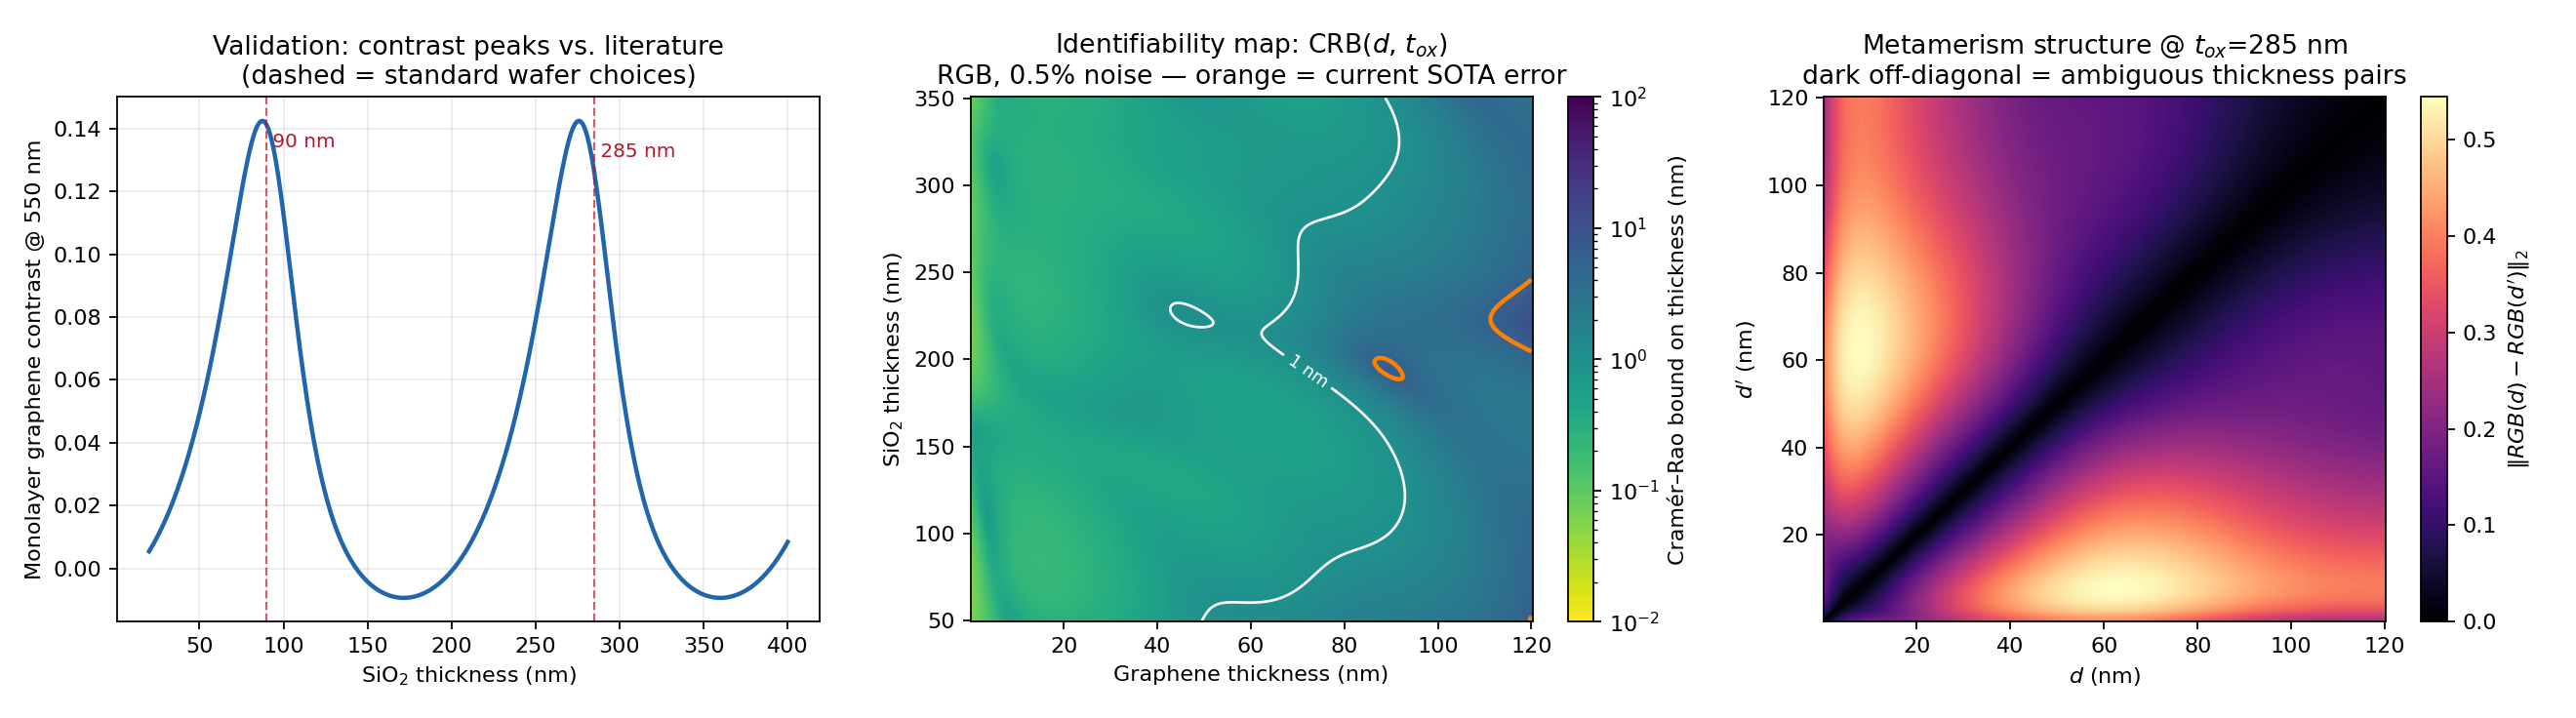
\includegraphics[width=\linewidth]{feasibility_study.png}
\caption{Forward-model validation and oracle identifiability. \emph{Convention:} this figure reports single-pixel oracle bounds (nuisances known), used only to establish the information floor of the measurement; all bounds quoted in the text and in Fig.~\ref{fig:crb} are prior-augmented and marginalized over the full nuisance set at 100 flake and 300 background pixels. \textbf{Left:} monolayer graphene contrast vs.\ oxide thickness (peak 0.142); dashed lines mark standard wafers. \textbf{Center:} oracle CRB over (thickness, oxide); orange contour = 5.8\,nm SOTA error, white = 1\,nm. \textbf{Right:} pairwise color distance at $t_{\mathrm{ox}}{=}285$\,nm; dark off-diagonal bands are ambiguous thickness pairs in the oracle setting.}
\label{fig:feas}
\end{figure}

\begin{figure}[t]
\centering
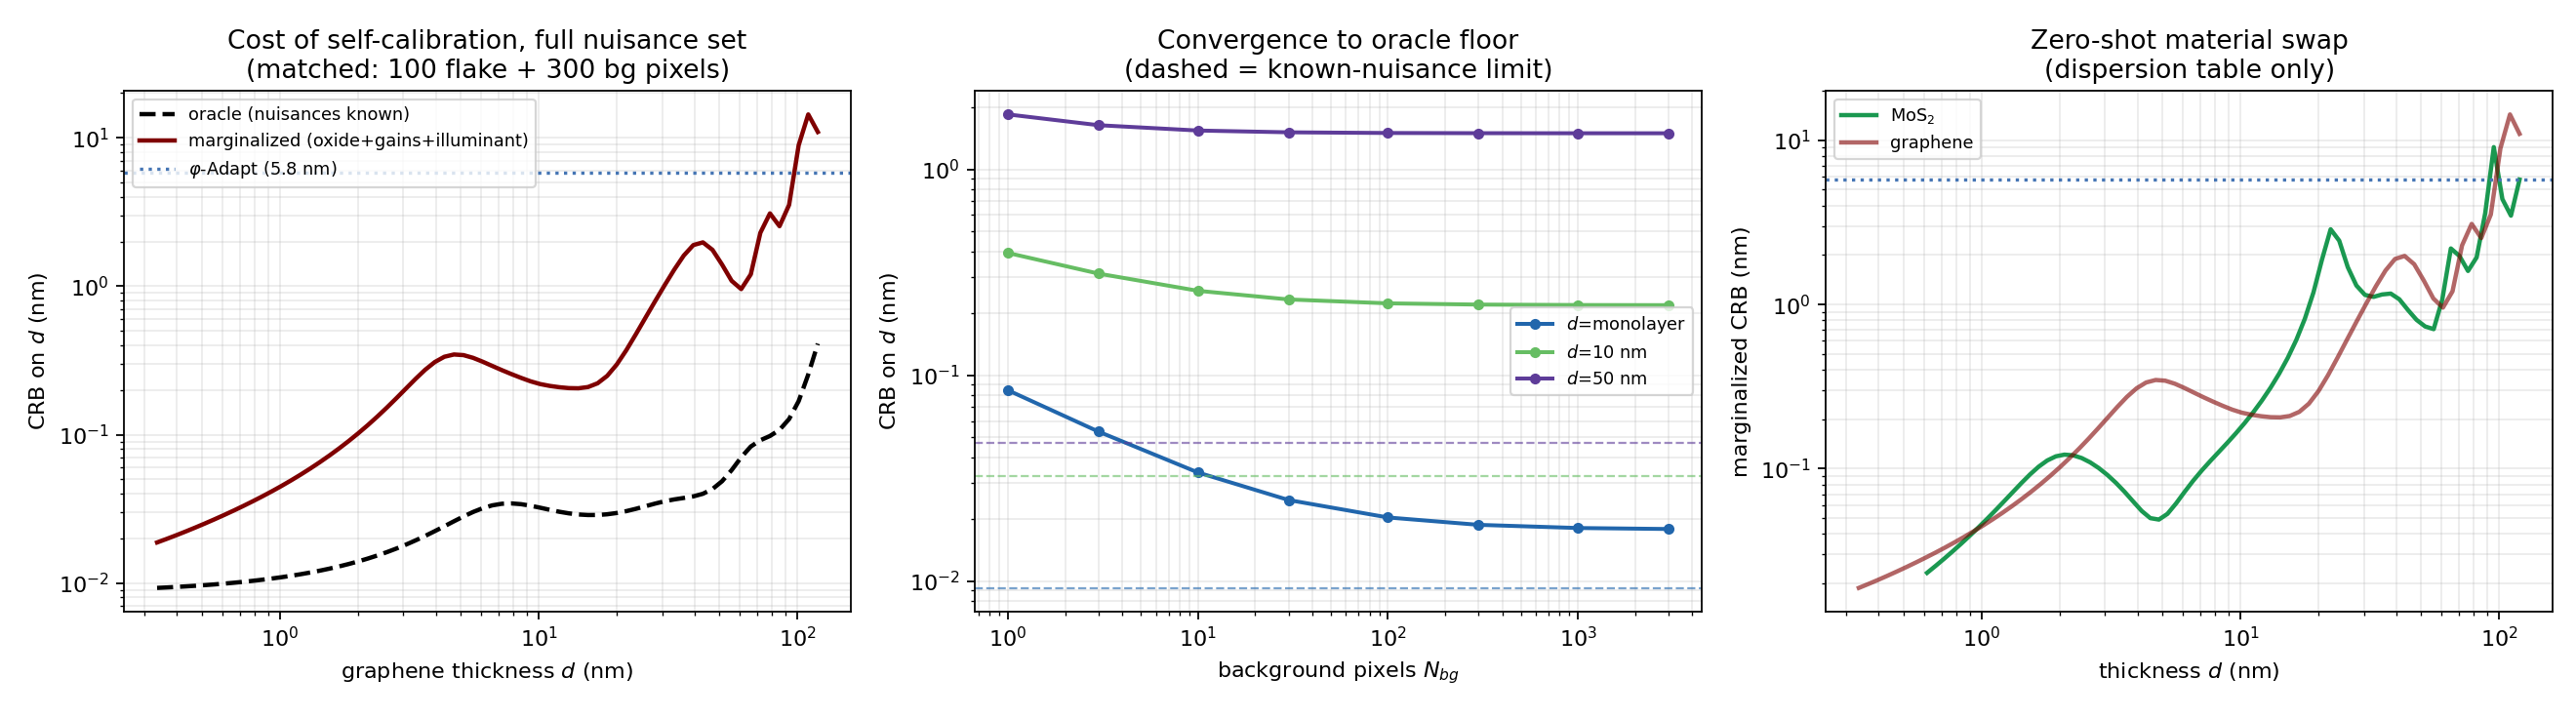
\includegraphics[width=\linewidth]{nuisance_crb.png}
\caption{The honest bound, computed with authoritative optical constants and the full nuisance set (oxide, gains, 5-component illuminant), matched at 100 flake and 300 background pixels. \textbf{Left:} oracle vs.\ fully marginalized CRB for graphene; the gap is the quantified price of self-calibration. \textbf{Center:} convergence toward the known-nuisance floor (dashed) as background evidence accumulates. \textbf{Right:} MoS$_2$ after a dispersion-table swap.}
\label{fig:crb}
\end{figure}

\subsection{The residual ambiguity is a joint ridge, not a metamer}\label{sec:ridges}

The failures that survive all single-frame improvements were assumed, by us and implicitly by the oracle analysis, to be classical metamers: two thicknesses producing the same color. Direct examination falsified this. On confidently-wrong scenes, the true thickness is \emph{not} close in color to the estimate at the fitted nuisances (gain-invariant ratio distances 0.08--0.27 against a noise scale of $\sim$0.006, with no rival minimum near the truth). Instead, the nuisance parameters drift \emph{continuously and jointly with thickness} along a ridge until the wrong interference order fits the frame essentially perfectly. Three natural mitigations fail for exactly this reason, and we verified each: ambiguity detection by counting posterior modes (the wrong solutions look unimodal --- 0 of 5 failures flagged); rival search by fixed-nuisance metamer scanning (finds nothing near the truth); and discrimination scores computed from fitted-mode color predictions (\S\ref{sec:negative}). The operative object is the \emph{profile posterior} $L^*(d)$, in which nuisances are re-optimized per thickness: the true solution appears there as a rival basin (typically 2--25 units above the wrong winner), which is what makes profile-based candidacy, triggering, and reporting sound. We advance this as a hypothesis with converging support rather than a settled theory: it rests on direct inspection of five failures plus the falsification of three mitigations it predicts should fail, and a larger diagnostic study would strengthen it.

\section{Experiments}\label{sec:experiments}

\subsection{Benchmark design}
Scenes are constructed to be \emph{hostile}: $d\sim$ log-uniform over $[1\ \mathrm{layer},120\,\mathrm{nm}]$; $t_{\mathrm{ox}}\sim\mathcal{N}(285,5^2)$; $\log g\sim\mathcal{N}(0,0.1^2)$; pixel noise $0.5\%$; $N_f{=}100$, $N_b{=}300$; and the illuminant drawn from the \emph{full eleven-spectrum family} (including spiky fluorescents) while the estimator has only the 5-component basis --- 1\% of illuminant variance is unmodelable by construction, so the benchmark contains genuine model misspecification rather than an inverse crime. We state plainly what this benchmark does \emph{not} test: oxide, gains, and noise are drawn from the estimator's own priors, so it is a well-specified Bayesian setting in those coordinates. We therefore add a \textbf{prior-violating stress test} in which oxide dispersion is $3\times$ the assumed prior ($\sigma{=}15$\,nm), gain dispersion $2.5\times$ ($\sigma_{\log g}{=}0.25$), and noise $2\times$ the assumed level: held-out median 0.203\,nm, mean 1.31\,nm, failures 5/60 (8.3\%), sub-25\,nm median 0.100\,nm ($n{=}60$, seed 205). Degradation is mild and self-calibration continues to recover the true oxide despite the mislabeled prior.

\subsection{Main results}
\textbf{Protocol.} To avoid selection effects, all design choices (mode window, positivity weight, basis size, solver schedule, grid density) were frozen after development on seeds $\{0,3,7,11\!-\!13,21,22,31\!-\!34,55,77,99\}$, and the numbers below were then produced on \emph{held-out} seeds $\{201\!-\!207\}$ never used for any decision. Held-out and development performance agree closely (median 0.104 vs.\ 0.123\,nm), indicating no overfitting to the development scenes.

Table~\ref{tab:main} and Fig.~\ref{fig:bench} report results. Our method's median appears at three values across this section --- 0.104\,nm (Table~\ref{tab:main}, seeds 201--202, $n{=}120$), 0.099\,nm (Table~\ref{tab:baselines}, the seed-201 subset, $n{=}60$, used so that baselines are compared on identical scenes) and 0.130\,nm (\S\ref{sec:masks}, seed 211, $n{=}40$) --- because these are the same estimator on different held-out subsets; the spread indicates the sampling variability to expect at these sample sizes. Median absolute error is \textbf{0.104\,nm} for graphene ($n{=}120$) and \textbf{0.154\,nm} for MoS$_2$ ($n{=}80$) with no retraining, fine-tuning, or labeled data of any kind --- the material swap is one dispersion table, against MaskTerial's 5--10 labeled images per material \cite{uslu2024maskterial}. In the sub-25\,nm regime, 1 of 148 held-out estimates failed (0/93 graphene; 1/55 MoS$_2$, where $d{=}10.4$\,nm was reported as 74.8\,nm).

\textbf{Comparison to the state of the art, stated carefully.} $\varphi$-Adapt reports a 5.8\,nm \emph{mean} error over 10--240\,nm \cite{phiadapt2025}, measured on 177 real flakes the authors collected for that purpose. That set is not public, so their number cannot be reproduced or re-run by us on identical data; this is a limit on the comparison that no amount of care on our side removes. Restricting our held-out scenes to the overlapping range ($d\ge10$\,nm, $n{=}47$) and using their metric, our mean error is 2.86\,nm: a $\mathbf{2.0\times}$ improvement. Other metric and range choices give much larger multipliers (full-range mean $4.9\times$; full-range median $56\times$), but we regard the range- and metric-matched figure as the only defensible headline. Even this restriction favors us: their range extends to 240\,nm while ours stops at 120\,nm, and the excluded band is precisely where our single-frame method is ridge-limited. Three caveats apply and none is minor: their number is measured on real images and ours on synthetic scenes; their pipeline includes segmentation error while ours assumes given regions; and their range extends beyond ours into the thick regime where our single-frame method is ridge-limited. \S\ref{sec:real} is the experiment that removes the first two.

\textbf{Identifiability and efficiency.} Two observations, made against per-scene bounds evaluated at each scene's \emph{true} parameters. First, the \emph{frequentist} CRB is unbounded: six numbers (two regions $\times$ three channels) cannot identify ten parameters, so the priors of \eqref{eq:map} are not a convenience but the reason the problem is well posed at all. Second, against the hybrid (prior-augmented) bound, achieved errors are at or below the bound --- median $|$error$|$/CRB of $0.28$ under real measured illuminants ($n{=}35$, thin regime) and $0.88$ when the illuminant is drawn from inside the estimator's basis span ($n{=}35$) --- versus $\approx\!0.67$ for an efficient unbiased estimator. We therefore claim only that \emph{the estimator is not the limiting factor}: a MAP estimator with informative priors is deliberately biased and the positivity constraint contributes information the linearized Fisher analysis omits, so sub-$0.67$ ratios are expected and this comparison is a diagnostic rather than a proof of efficiency. We flag that an earlier version of this analysis, which linearized the bound at illuminant coefficients recovered under a mismatched normalization (up to $327\sigma$ from the prior, i.e.\ at physically invalid spectra), produced ratios near 10 and supported the opposite conclusion; the corrected analysis supersedes it.

\textbf{Robustness to illuminants outside the model family.} The spectral basis is a PCA over eleven measured illuminants, and both it and the benchmark draw on that family, so we tested illuminants of entirely different physical type: blackbody sources at 2800/3400\,K, a xenon arc, a narrow-band high-CRI LED, and a mercury arc with strong emission lines (26--39\% of their spectral deviation is unrepresentable in the basis, against 9\% for in-family sources). Thin-regime performance is essentially unaffected: median errors 0.030--0.109\,nm, worst-case 1.30\,nm, and \textbf{zero failures in 64 estimates} (16 per illuminant). The explanation is structural, and worth stating precisely. For a fixed stack, each observed channel is a \emph{ratio} of linear functionals of the illuminant: a numerator $\int L(\lambda)R(\lambda)\bar{x}_i(\lambda)\,d\lambda$ and a common normalizer $\int L\bar{y}$. A two-region scene thus depends on $L$ through six numerator functionals and one normalizer; the normalizer is a global scale that the per-channel gains absorb, leaving the illuminant identifiable only up to a projection onto a subspace of dimension at most six. Components of $L$ outside that subspace cannot influence the fit, whatever their magnitude. A basis need only span the \emph{identifiable projection}, not the spectrum itself, which is why a five-component basis plus three gains absorbs a mercury arc whose spectral deviation is 39\% unrepresentable. This also predicts the limit of the argument: acquiring a second frame through a known filter (\S\ref{sec:protocols}) enlarges the identifiable subspace, which is precisely why that protocol works. This is a stronger robustness result than in-family testing could establish, and it removes spectral misspecification as a leading concern for real deployment.

\begin{table}[t]
\centering
\caption{Held-out benchmark (frozen configuration, seeds never used in development). Failures are errors ${>}5.8$\,nm; 95\% CIs are Clopper--Pearson. ``v1'' is the multi-start first-order ablation of our own estimator (\S\ref{sec:negative}), evaluated on development seeds.}
\label{tab:main}
\begin{tabular}{lccc}
\toprule
 & Graphene ($n{=}120$) & MoS$_2$ zero-shot ($n{=}80$) & Graphene, v1 ablation \\
\midrule
Median $|$error$|$ & \textbf{0.104}\,nm & \textbf{0.154}\,nm & 0.276\,nm \\
Mean $|$error$|$ & 1.19\,nm & 1.95\,nm & 2.85\,nm \\
Mean, $d\ge10$\,nm (SOTA range) & 2.86\,nm & --- & --- \\
Median, $d<25$\,nm & \textbf{0.055}\,nm & \textbf{0.073}\,nm & 0.153\,nm \\
Failures & 8/120 (6.7\%, CI [2.9, 12.7]) & 4/80 (5.0\%, CI [1.4, 12.3]) & 17/120 \\
Failures, $d<25$\,nm & 0/93 & 1/55 & 0/90 \\
Time / flake (CPU) & 1.5\,s & 1.5\,s & 3.5\,s \\
\bottomrule
\end{tabular}
\end{table}

\begin{figure}[t]
\centering
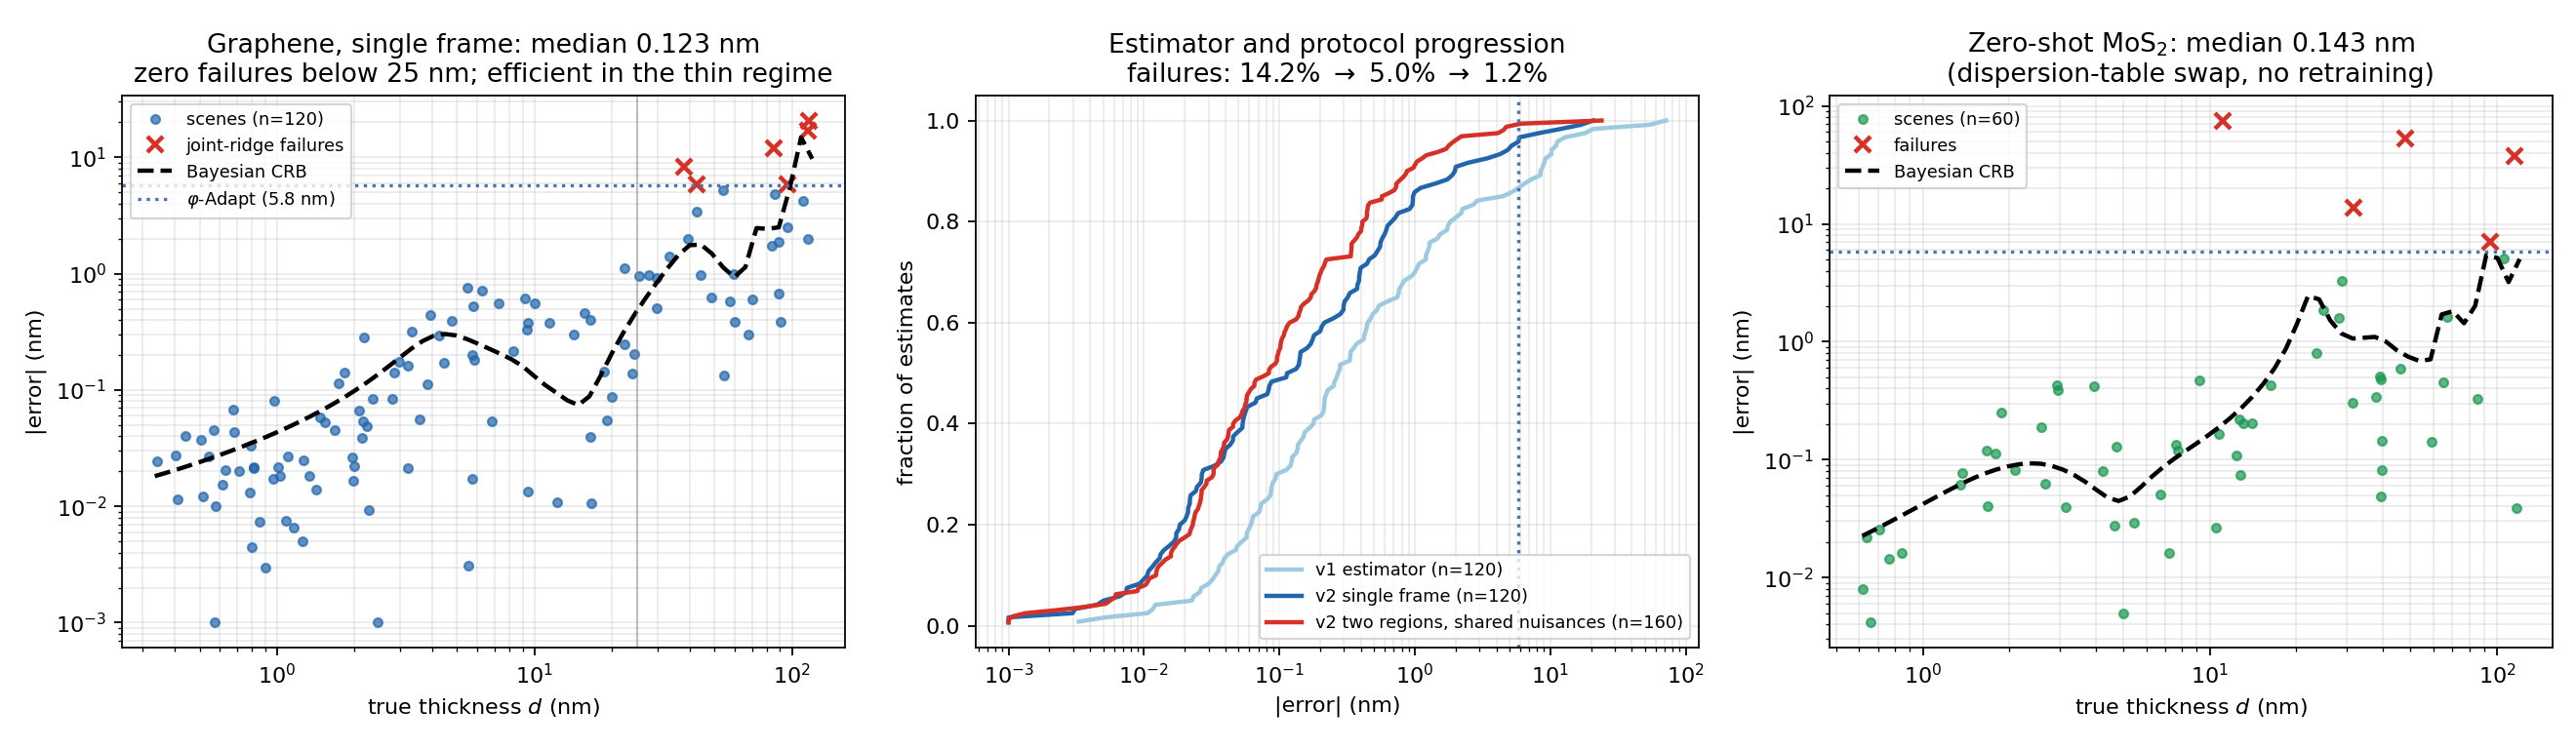
\includegraphics[width=\linewidth]{benchmark_results.png}
\caption{Results. \textbf{Left:} graphene errors vs.\ truth against the Bayesian CRB; all failures (red) lie beyond 25\,nm in the joint-ridge domain. \textbf{Center:} error CDFs across estimator generations and the multi-region protocol. \textbf{Right:} zero-shot MoS$_2$.}
\label{fig:bench}
\end{figure}

\subsection{Layer counting, the field's own metric}\label{sec:layers}
Prior systems report discrete layer classes, so for direct comparability we convert our continuous estimates to the nearest integer layer count. Real flakes are integer multiples of the layer height, so we evaluate on scenes whose thickness is exactly $n\times0.335$\,nm, $n\in[1,10]$ (an earlier version of this analysis used the log-uniform continuous thicknesses of the main benchmark, which is not physical and understated accuracy). On 45 such scenes graphene achieves \textbf{82.2\% exact} layer accuracy and \textbf{100\% within one layer}, with a median error of 0.15 layers (0.050\,nm). Exact accuracy is layer-dependent (100\% at 1--2 layers, 90.9\% at 3--5, 70.8\% at 6--10) because its 0.335\,nm interlayer spacing makes adjacent classes increasingly hard to separate as thickness grows. MoS$_2$, with nearly double the layer height, is correspondingly easier.

The monolayer case, which is what most exfoliation searches are actually looking for, is the strongest result in the paper: median absolute error of \textbf{0.0146\,nm for monolayer graphene} and \textbf{0.0114\,nm for monolayer MoS$_2$}, i.e.\ 0.04 and 0.02 of a layer respectively. Discrete classification cannot express this: the method does not merely place a monolayer in the right bin, it measures it to a few percent of an atomic layer.

\subsection{Comparison to simpler approaches}\label{sec:baselines}
To establish how much of the performance comes from the full machinery rather than from correct physics alone, we compare against three progressively simpler methods on identical held-out scenes ($n{=}60$, seed 201): \textbf{B1}, gain-invariant contrast lookup against a curve precomputed at \emph{nominal} nuisances, i.e.\ the calibrated-contrast approach used in the field but \emph{without} per-setup calibration, and involving no optimization; \textbf{B2}, optimizing thickness alone with nuisances pinned at prior means; and \textbf{B3}, optimizing thickness and the three channel gains, i.e.\ conventional white-balance correction without oxide or illuminant estimation. We additionally report \textbf{B1-oracle}, the same lookup given the \emph{true} oxide thickness and the \emph{true} illuminant spectrum of each scene. B1-oracle is not achievable in practice, since it presumes exact knowledge of the illuminant SPD, but it bounds what any method could attain if imaging conditions were known, and it is the reference against which self-calibration should be judged. B2 and B3 are given 24 multi-start Levenberg--Marquardt fits; their parameter spaces are one- and four-dimensional respectively, so they are not optimizer-limited.

\begin{table}[h]
\centering
\caption{Ablation against simpler methods, identical held-out scenes ($n{=}60$).}
\label{tab:baselines}
\begin{tabular}{lcccc}
\toprule
 & Median $|$err$|$ & Mean $|$err$|$ & Failures & Median, $d<25$\,nm \\
\midrule
B1 contrast lookup (field standard) & 0.253\,nm & 5.77\,nm & 11/60 & 0.105\,nm \\
B2 fixed nuisances & 1.883\,nm & 11.84\,nm & 20/60 & 1.044\,nm \\
B3 gain-only calibration & 0.516\,nm & 5.03\,nm & 12/60 & 0.197\,nm \\
\textbf{Ours (full joint estimation)} & \textbf{0.099}\,nm & \textbf{1.77}\,nm & \textbf{6/60} & \textbf{0.037}\,nm \\
\midrule
\emph{B1-oracle} (true oxide + illuminant; & \emph{0.020}\,nm & \emph{0.13}\,nm & \emph{0/45} & \emph{0.015}\,nm \\
\quad unachievable upper bound) & & & \emph{CI [0, 7.9]\%} & \\
\bottomrule
\end{tabular}
\end{table}

Correct physics alone (B1) is already competitive in median error, which is why calibrated-contrast methods work as well as they do in practice; but its mean error and failure rate are 3--4$\times$ and 2$\times$ worse, because it has no way to absorb imaging-condition variation. Pinning nuisances (B2) is worst of all, confirming that estimating them matters more than optimizing carefully. Gains alone (B3) recover part of the gap. Full joint estimation improves median error by $2.6\times$ over uncalibrated lookup and $5\times$ over white-balance correction, and halves the failure rate. The self-calibration mechanism, not the optimizer, is the source of the gain.

The B1-oracle row frames this result properly and we state it plainly: \emph{if imaging conditions were known, a trivial lookup table would beat our method by a factor of five} (median 0.020 vs.\ 0.101\,nm; on paired scenes B1-oracle is better on 37 of 45). Our method does not compete with knowing the answer; it competes with not knowing it. Reading the three regimes together --- uncalibrated lookup 0.253\,nm, ours 0.101\,nm, oracle-calibrated lookup 0.020\,nm --- self-calibration recovers roughly 65\% of the gap between having no calibration and having perfect calibration, while requiring no reference samples, no known-thickness standards, and no per-setup procedure. This comparison also provides an \emph{independent check on the identifiability theory of \S\ref{sec:theory}}, which matters because the bounds and the estimator share no code path: B1-oracle is a 600-point table lookup, while the bounds come from automatic differentiation of the forward model. For Gaussian errors $\mathrm{median}|e|=0.6745\,\sigma$, so B1-oracle's median error of 0.0204\,nm implies $\sigma=0.0302$\,nm against a predicted oracle bound of 0.0289\,nm, an agreement of $1.05\times$: the oracle lookup is statistically efficient and the Fisher computation is corroborated. Our method's median of 0.1014\,nm implies $\sigma=0.150$\,nm against a full-nuisance bound of 0.233\,nm, a ratio of 0.64, consistent with the per-scene analysis in \S\ref{sec:experiments} and with the shrinkage expected of a MAP estimator under informative priors. The residual 35\% is the price of inferring imaging conditions from the image itself, and it is the quantity a spectrally richer acquisition (\S\ref{sec:protocols}) is designed to reduce.

\subsection{Coverage: alternate substrate and a transparent material}\label{sec:coverage}
The main benchmark uses 285\,nm oxide and two absorbing materials. We add the other standard wafer and the field's acknowledged hard case. \textbf{90\,nm oxide} (graphene, $n{=}40$): median 0.052\,nm, mean 1.30\,nm, 3/40 failures (7.5\%, 95\% CI [1.6, 20.4]), 0/28 below 25\,nm. \textbf{hBN on 285\,nm oxide} ($n{=}40$), which is transparent in the visible ($k{=}0$) so that contrast arises from phase alone and which MaskTerial identifies as its difficult low-contrast case: median 0.113\,nm, mean 0.531\,nm, \textbf{0/40 failures} (95\% CI [0, 8.8]\%). A physics-based estimator is not disadvantaged by low contrast in the way a contrast classifier is, because the thickness information resides in the interference phase rather than in contrast magnitude.

\subsection{Sensitivity to the assumed optical constants}\label{sec:nk}
The forward model treats the material's dispersion as known, yet tabulated $n,k$ for 2D materials disagree between sources by more than a few percent, and graphene's constant-index model is itself an approximation. We render scenes with $n$ and $k$ scaled by $(1{+}\varepsilon)$ while the estimator retains the nominal values ($n{=}30$ per setting). At $\varepsilon{=}2\%$: median error 0.407\,nm, 0/30 failures, sub-25\,nm median 0.079\,nm. At $5\%$: 1.076\,nm, 5/30 failures, sub-25\,nm 0.183\,nm. At $10\%$: 1.785\,nm, 10/30 failures, sub-25\,nm 0.349\,nm.

Two features matter. The error is \emph{systematically signed} (median $+0.095$, $+0.180$, $+0.328$\,nm), as expected: an overestimated refractive index is compensated by an overestimated thickness, so dispersion error appears as a calibration offset rather than as noise. And the thin regime is far more robust than the thick one, staying sub-nanometre even at $10\%$ dispersion error, while failures concentrate above 25\,nm where ridges already exist. Practically this means the method inherits the accuracy of its dispersion table in the thick regime and should be paired with material-specific tabulated data rather than constant-index approximations when absolute accuracy beyond a few nanometres is required. Estimating $n,k$ jointly is possible in principle given enough regions sharing one material, and is the natural extension.

\subsection{Sensitivity to imperfect segmentation}\label{sec:masks}
Since we assume given regions (\S1), we quantify the cost of mask error by mixing a fraction $\alpha$ of substrate signal into the flake region, as a dilated or leaky mask would (graphene, $n{=}40$ per setting, seed 211). Median error rises from 0.130\,nm at $\alpha{=}0$ to 0.135 ($\alpha{=}2\%$), 0.226 ($5\%$), 0.280 ($10\%$) and 0.502\,nm ($20\%$), with failures 2, 2, 2, 1 and 4 of 40 (95\% CI at $\alpha{=}20\%$: [2.8, 23.7]\%). Degradation is graceful and sub-nanometre accuracy survives 20\% contamination, but an end-to-end system would inherit its segmenter's error on top of this, and we have not measured that composition.

\subsection{Acquisition protocols for the thick regime}\label{sec:protocols}
All remaining failures pair the truth with a joint-ridge partner beyond 25\,nm. Because the ambiguity is information-theoretic for a single frame, the remedies are acquisition protocols, each derived from the theory and each costing almost nothing in practice. We report these on 25--80 scenes; they establish large effects, not the absence of failure, and the confidence intervals below should be read as the operative claim:

\textbf{Multi-region (mode lattice).} On 80 two-region scenes (160 estimates; development seeds, not held-out): median 0.084\,nm, failures $9.4\%\!\to\!\mathbf{1.3\%}$ overall and $41.7\%\!\to\!\mathbf{5.6\%}$ in the hard $d{>}25$\,nm regime relative to the v1 joint search, at $2.7\times$ lower cost. Three regions, in an all-hard-regime stress test (every $d\in[28,120]$\,nm): \textbf{0/60 failures} (95\% CI [0\%, 6.0\%]), median 0.27\,nm, versus 7/60 for single-frame estimation of the same regions.

\textbf{Known-filter two-frame protocol.} A second photograph of the same field through a known color filter (an inexpensive gel; we model a smooth long-pass with 0.12 floor), with illuminant coefficients \emph{shared} across frames and per-frame gains, converts two RGB frames into coarse spectroscopy: hard-regime failures $3/25\to\mathbf{0/25}$ (95\% CI [0\%, 13.7\%]; the sample is small and we report it as strong evidence of a large effect, not as a demonstration of exactly zero failure probability). The control experiment matters: two frames under two \emph{unknown} illuminants barely help ($5/25\to4/25$), because each frame's unknown spectrum hands the wrong ridge fresh nuisance freedom --- the spectral change must be \emph{known}.

\textbf{Profile-triggered acquisition.} The second frame is requested only when the profile posterior shows any rival basin within a wide trigger window (40 units). On hard-regime scenes this fired 11/25 times and caught the confidently-wrong cases that mode-count triggers miss entirely (\S\ref{sec:ridges}); on the standard benchmark the vast majority of scenes are certified unimodal and need one frame.

\subsection{Numerical aperture: the dominant systematic, and a hard requirement}\label{sec:na}
Real objectives illuminate over a cone. We implement oblique-incidence TMM (s/p characteristic matrices, pupil-uniform quadrature in $\sin^2\theta$), validated to machine precision against \cite{byrnes2016} at angle. This turns out to be the single most consequential modeling choice in the paper, and we report it plainly because our own first analysis of it was wrong.

\textbf{NA sets the contrast-optimal substrate.} The oxide thickness maximizing monolayer contrast at 550\,nm moves from 88/276\,nm at normal incidence to 90/286 (NA\,0.55), 94/296 (NA\,0.75) and 96/304\,nm (NA\,0.90). Flake-hunting objectives are typically 50--100$\times$ with NA\,0.55--0.9, and at those apertures the model reproduces the community's standard 90\,nm and 285--300\,nm wafers. Magnitudes agree too: on 300\,nm oxide at 550\,nm our NA\,0.9 contrast is 0.090, inside the 0.09--0.12 range reported by Blake et al.\ \cite{blake2007} using a 100$\times$/0.9 objective, whereas the normal-incidence value of 0.063 is well below it. The standard wafers are not folklore; they are correct for the optics actually used, and reproducing them at the right NA is an independent validation of our forward model.

\textbf{Mismatched NA is catastrophic, including where we otherwise never fail.} Rendering truth at NA\,0.90 and estimating with a normal-incidence model gives median error 1.53\,nm, mean 5.56\,nm, 11/30 failures, and \textbf{5/21 failures below 25\,nm} --- the only setting anywhere in this paper that produces sub-25\,nm failures. At NA\,0.55 the same mismatch is benign (median 0.097\,nm, no failures), which is why a first pass at moderate aperture badly understated the risk. Matching the forward model to the objective removes the problem entirely: at NA\,0.90 with an NA-aware estimator, median error is 0.026\,nm with 0/12 sub-25\,nm failures.

\textbf{Requirement, not a refinement.} The numerical aperture of the objective must be known and built into the forward model. This is a one-line change and the value is engraved on every objective, but omitting it silently destroys thin-regime accuracy. Pupil quadrature needs $\ge6$ nodes for metrology-grade use, at roughly $6$--$10\times$ the forward-model cost.

\subsection{Robustness}\label{sec:robust}
\textbf{8-bit imagery.} Real micrographs arrive quantized. Encoding each pixel to sRGB, rounding to 8 bits, adding read noise and averaging over the region reproduces the continuous-input result: median 0.051\,nm, sub-25\,nm median 0.042\,nm, 0/30 failures ($n{=}30$, 100 flake pixels). Quantization is dithered away by read noise and is not a limiting factor. We note one caution: averaging 1000 rather than 100 pixels did not improve the median (0.231 vs.\ 0.051\,nm on $n{=}30$), consistent with a small quantization-induced bias floor that further averaging cannot reduce; the sample is small and this deserves confirmation on real data.

With the noise model mis-set by $2\times$ and $4\times$ (truth noisier than assumed): medians 0.087/0.120\,nm, zero failures. With the wafer mislabeled by $3\sigma$ (true oxide $\mathcal{N}(300,5)$\,nm against a 285\,nm prior): median 0.128\,nm, 1/20 failures --- self-calibration recovers the true oxide from the data and overrides the label.

\subsection{Negative results and ablations}\label{sec:negative}
We report what failed, verified pairwise on identical scenes. (1) \emph{First-order multi-start} (32 Adam \cite{kingma2015} restarts; ``v1'' in Table~\ref{tab:main}): the accuracy gap to the continuation estimator traces to underconvergence and non-exhaustive mode discovery. (2) \emph{Closed-form gain marginalization} (Rao--Blackwellization): mathematically exact, empirically worse (mean error 2.06 vs.\ 1.01\,nm, two new failures) and slower --- profiling gains degrades the Gauss--Newton geometry and permits negative gains. (3) \emph{Richer illuminant basis alone} (5 vs.\ 3 components, before the positivity constraint and dual-start solves): a wash --- fixed 6 failures, introduced 7; added flexibility helps wrong ridges as much as right ones. The accuracy gains in this paper come from the diagnosed physical constraints, not from added capacity. \emph{Statistical caveat:} we tested these design decisions by paired comparison on 120 scenes, where failures are rare events. Only the aggregate first-order-to-continuation change is significant (11 failures fixed, 0 introduced; exact McNemar $p{=}0.001$); the individual accept/reject decisions above rest on differences of 1--7 failures that are \emph{not} statistically distinguishable from noise ($p\ge0.13$). We report them as engineering judgements supported by mechanism, not as established effects. (4) \emph{Adaptive filter selection}: choosing the frame-2 filter by maximizing predicted mode separation was unreliable --- on the one scene where choice mattered, the score's top-ranked filter failed (101.1\,nm vs.\ truth 94.0) while its worst-ranked filter succeeded (94.7\,nm), because the score is computed from drifted-nuisance predictions (\S\ref{sec:ridges}). The validated protocol is the trigger plus a fixed known filter; ridge-aware selection is future work.

\subsection{Real-data evaluation on public micrographs}\label{sec:real}
We evaluate on the public MaskTerial \texttt{GrapheneL} dataset \cite{uslu2024maskterial}: real reflected-light micrographs of exfoliated graphene with per-pixel layer annotations, acquired on a $20\times$ objective by a different laboratory with no involvement from us. The objective is a CFI TU Plan Fluor EPI $20\times$ at NA\,0.45 \cite{uslu2024gmm}, and the forward model is NA-averaged at that aperture throughout this section; the high-aperture failure of \S\ref{sec:na} therefore does not arise on this corpus, which sits in the regime where a normal-incidence approximation is benign. Flake and substrate regions are taken from the released semantic masks; no other preprocessing is applied.

\textbf{The substrate is coloured, as the physics requires, and the joint estimate is nonetheless ridge-limited.} The forward model predicts a strongly blue bare wafer at $90$\,nm oxide (linear RGB $[0.110,0.098,0.177]$, $B/R=1.61$), and the released \texttt{GrapheneL} images agree qualitatively: the bare wafer measured over all $1362$ test images reads $[113,107,151]$ ($B/R=1.34$) with an inter-image IQR of $[64,10,69]$. The substrate term of \eqref{eq:map} therefore carries information here, and the self-calibration mechanism is not vacuous on this dataset. What limits the full joint estimate instead is the ridge structure of \S\ref{sec:ridges}: per-flake inversion places a minority of flakes in a spurious basin near $35$--$41$\,nm oxide, at a rate that varies by exfoliation run. We therefore report both modes below: the full joint estimate, which recovers the wafer, and a restricted mode, which is more reliable for per-flake layer counting.

\textbf{A restricted mode trades the per-flake ridge for a per-dataset assumption.} Pinning the illuminant and treating the oxide as a single global constant per dataset removes the per-flake nuisance freedom that the ridge exploits: it leaves the substrate determining the three gains exactly ($3$ equations, $3$ unknowns) and the flake determining one thickness from three observations. The oxide is calibrated once on the \emph{train} split and the \emph{test} split is then evaluated without further adjustment. This is the physical analogue of the adaptation baselines perform: MaskTerial requires 5--10 labeled images per material \cite{uslu2024maskterial}; we require one scalar. The cost is that a single global oxide is only appropriate when a dataset is a single wafer, which these are not (Table~\ref{tab:cross}); the full joint estimate makes no such assumption and is reported alongside it.

\textbf{The gain prior is an operating parameter on real images, not a frozen constant.} The log-gain prior width $\sigma_g{=}0.1$ of \eqref{eq:map} is correct on the synthetic benchmark by construction, since gains there are drawn from it. On real micrographs the overall exposure is physically arbitrary and well determined by the data: it fits at $4.35$ on \texttt{Set\_Graphene-Jan3-22-04-2022} regardless of the prior, which at $\sigma_g{=}0.1$ is a $21\sigma$ penalty on a quantity the model has no business constraining. Widening to $\sigma_g{=}1.5$ on the same 39 flakes tightens the label-free fitted-oxide scatter from $7.13$ to $5.22$\,nm (MAD) and moves the chromatic ratios toward neutral ($R/G$ $0.98{\to}0.90$, $B/G$ $0.81{\to}0.92$), while leaving the ridge untouched --- the failures that remain are the same joint-mode failures, unchanged in character. Ridge failures fall $38.5\%{\to}30.8\%$ (4 fixed, 1 introduced), which by the standard of \S\ref{sec:negative} is not a demonstrated effect (exact McNemar $p{=}0.375$). We therefore report $\sigma_g{=}1.5$ as a documented setting for acquisitions of unknown exposure rather than changing the frozen default, and note that the reparameterization this suggests --- factoring the gains into a free exposure scale and a priored chromatic balance --- is the principled version and is untested here.

\textbf{Two acquisition parameters are recovered from the images themselves.} Sweeping oxide thickness over $60$--$320$\,nm produces a single sharp global minimum in color-fit residual at $90$\,nm (neighboring candidates are $2.5$--$9\times$ worse), recovering the standard graphene wafer specification without being told it. Separately, testing sRGB versus linear decoding showed the released images are radiometrically linear rather than sRGB-encoded, a fact not stated in the dataset documentation: assuming sRGB inflated recovered thickness by a factor $2.19$ and produced a residual that grew with thickness, while linear decoding simultaneously reduced the residual, moved the recovered oxide to nominal, and collapsed the scale error to $0.6\%$. Four independent diagnostics moving together is what distinguishes a physical correction from a tuned parameter.

\textbf{Result on the held-out test split} ($n{=}200$ flakes, 1--4 layers) is given in Table~\ref{tab:real}:

\begin{table}[h]
\centering
\caption{Real-data evaluation, MaskTerial \texttt{GrapheneL} test split. Oxide calibrated on the train split only; no labeled examples used for training.}
\label{tab:real}
\begin{tabular}{lc}
\toprule
Exact layer agreement & \textbf{97.0\%} (95\% CI [94.5, 99.0]) \\
Within one layer & \textbf{100.0\%} \\
Recovered layer height & $0.3380 \pm 0.0043$\,nm/layer (true $0.335$; error $+0.9\%$) \\
Intercept & $+0.029$\,nm \\
Correlation with annotation & $r = 0.9847$ \\
Flakes with poor individual color fit & 4/200 \\
Per-class exact agreement & 98.4 / 95.7 / 95.1 / 100.0\% (1/2/3/4 layers) \\
\bottomrule
\end{tabular}
\end{table}

\textbf{The recovered slope is a physical thickness scale, not an ordering of the supplied labels.} This is the substantive claim of the real-data experiment and we state it explicitly, because the natural objection is that agreement with optically-derived annotations could reflect nothing more than reproducing their rank order. Across held-out real images the inferred thickness rises by $0.3380 \pm 0.0043$\,nm per annotated layer on \texttt{GrapheneL} and $0.3388 \pm 0.0054$\,nm on the independent \texttt{GrapheneM} acquisition, agreeing with graphene's independently known $0.335$\,nm interlayer spacing to $0.9\%$ and $1.1\%$ respectively. A method that had learned only to rank the annotations would have no reason to reproduce that constant, and none to reproduce it twice from two acquisitions that yield different substrate thicknesses. The interlayer spacing is not supplied to the estimator at any point; it is an output. What this does \emph{not} establish is per-flake accuracy against an independent physical measurement, which requires AFM or Raman and remains the necessary next test.

\textbf{What this does and does not establish.} The annotations are layer classes assigned from optical images, so agreement demonstrates that we reproduce the community's labeling on the community's data, not agreement with an independent physical measurement; AFM or Raman validation remains future work. The residual still grows with thickness ($0.036 \to 0.099$ across classes) and the log-log exponent is $0.977 \pm 0.011$, marginally excluding pure proportionality, so a small unmodelled nonlinearity remains in their pipeline. Results are reported for one material on one dataset over 1--4 layers.

\textbf{Transfer across the designed substrate-variance series.} MaskTerial ships graphene as \texttt{GrapheneL/M/H}, which are not three acquisitions but three samplings of one pool of named exfoliation runs, constructed by their authors to span approximately $5$, $10$ and $20$\,nm of oxide thickness about a nominal ${\sim}90$\,nm wafer \cite{uslu2024maskterial}. They overlap: \texttt{GrapheneL} and \texttt{GrapheneM} share 162 images, byte-identical where they overlap. We apply an identical command to each: oxide and transfer function re-derived from each dataset's own images, no labeled examples, no per-dataset tuning. Our restricted mode represents each by a single global oxide, an assumption the series progressively violates by design, so Table~\ref{tab:cross} measures robustness to substrate spread rather than transfer between laboratories.

\begin{table}[h]
\centering
\caption{Transfer across the MaskTerial graphene substrate-variance series. \texttt{L}, \texttt{M} and \texttt{H} denote low, medium and high substrate-thickness variance: the datasets were built by their authors to span ${\sim}5$, ${\sim}10$ and ${\sim}20$\,nm of oxide about a nominal ${\sim}90$\,nm wafer \cite{uslu2024maskterial}, and they draw on a shared pool of exfoliation runs rather than being independent acquisitions. Oxide recovered from each dataset's own images without labels, by minimizing color-fit residual over a 60--320\,nm sweep; transfer function selected from the images; nothing tuned per dataset. The fitted oxide is a mixture-weighted compromise over the nine or ten runs each dataset contains, not a wafer measurement. The $n{=}600$ row reuses the oxide recovered from the $n{=}200$ \texttt{GrapheneL} scan and is a larger draw from the same pool. Intervals are bootstrap 95\% CIs (4000 replicates).}
\label{tab:cross}
\begin{tabular}{lcccc}
\toprule
Dataset & Oxide & Exact agreement & Recovered layer height (nm) & $r$ \\
\midrule
\texttt{GrapheneL} ($n{=}600$) & 92\,nm & 95.3\% [93.7, 96.8] & $0.3370$ [0.3310, 0.3439] & 0.974 \\
\texttt{GrapheneL} ($n{=}200$) & 92\,nm & 97.0\% [94.5, 99.0] & $0.3380$ [0.3316, 0.3449] & 0.985 \\
\texttt{GrapheneM} ($n{=}200$) & 96\,nm & 93.5\% [90.0, 96.5] & $0.3388$ [0.3284, 0.3489] & 0.976 \\
\texttt{GrapheneH} ($n{=}200$) & 98\,nm & 76.5\% [70.5, 82.0] & $0.2904$ [0.2694, 0.3102] & 0.892 \\
\bottomrule
\end{tabular}
\end{table}

\textbf{The recovered slope is a physical thickness scale, not an ordering of the supplied labels.} This distinction is the natural objection to any evaluation scored against annotations, and the data answers it directly: across the held-out real images the inferred thickness increases by $0.3370 \pm 0.0032$\,nm per annotated layer ($n{=}600$), in agreement with graphene's independently known $0.335$\,nm interlayer spacing to $0.6\%$. A method that had learned only to reproduce the community's labeling would order flakes correctly but carry no obligation to recover that constant; the constant is a property of the crystal, is nowhere supplied to the estimator, and enters only through the tabulated optical dispersion. We are careful about what this does and does not establish: it demonstrates that the \emph{scale} of the recovered thicknesses is physically correct, not that any individual flake has been measured against an independent instrument. Per-flake validation against AFM or Raman remains the necessary next experiment (\S\ref{sec:limitations-note}).

\textbf{The recovered spacing is consistent across the series to within sampling noise.} Graphene's $0.335$\,nm lies inside the confidence interval for \texttt{GrapheneL} and \texttt{GrapheneM}, and every pairwise bootstrap comparison among them is consistent (\texttt{L}$_{600}$ vs.\ \texttt{M}: $-0.0018$\,nm, CI $[-0.0134,+0.0110]$). We stress that these are \emph{not} independent acquisitions: \texttt{GrapheneL} and \texttt{GrapheneM} share 162 images, byte-identical where they overlap, and each dataset is itself a sampling from a shared pool of named exfoliation runs. The fitted values of 92, 96 and 98\,nm are accordingly mixture-weighted compromises over the nine or ten runs each dataset contains, not three wafer measurements; the upward drift with the series' designed oxide spread is the expected behaviour of a single-oxide fit to a broadening distribution. Per-run fits are reported below and are the meaningful wafer estimates.

Two robustness checks accompany this. The bootstrap CI half-width on layer height falls from $\pm10.9\%$ at $n{=}25$ to $\pm2.0\%$ at $n{=}600$, scaling as $n^{-1/2}$, so the residual error is statistical rather than systematic and more flakes would tighten it further. Varying the mask-erosion depth from 1 to 6 pixels changes the recovered layer height by under $2\%$ on both \texttt{GrapheneL} ($0.3355$--$0.3402$) and \texttt{GrapheneM} ($0.3341$--$0.3410$), within the sampling interval, so the one free preprocessing parameter is not driving the result.

\texttt{GrapheneH} differs from all three with CIs excluding zero, reading $13\%$ low with the deficit concentrated in its thicker classes; within-one-layer agreement remains $97.5\%$, so ordering is preserved and only absolute scale degrades. We report it rather than the best two. Notably its color-fit residual is the \emph{lowest} of the four, so the self-diagnosis does not flag it --- bounding what that check can be trusted to catch: it detects images the physics cannot explain, not annotations that disagree with the physics.

\textbf{Materials where the method refuses, and one where the labels are the puzzle.} Applying the same command to the released TMD datasets, the color-fit criterion rejects both: \texttt{WSe2} (residual $0.336$, recovered layer height $-21.8\%$, 120/135 flakes individually flagged) and \texttt{MoSe2} (residual $0.125$, $+64.7\%$, 35/95 flagged). These are correct refusals. We stress that \texttt{MoSe2} simultaneously reports $100\%$ ``exact agreement'', because with only two label classes and a systematic scale error, rounding lands correctly --- a demonstration that the field's standard classification metric can appear perfect while the underlying physics is wrong, and an argument for reporting a physical consistency check alongside it.

\texttt{hBN\_Thin} is also the one dataset in which our substrate-calibration assumption genuinely fails, and it is worth separating that from the layer-height question. Its bare wafer reads neutral grey (median RGB $[156,159,154]$) with an inter-image IQR of $[2.0,2.2,0.2]$, whereas the physics predicts a strongly coloured substrate at any oxide in its range. The camera was evidently white-balanced on the substrate, which is standard microscopy practice. Three free channel gains can then reproduce \emph{any} substrate color, so the bare-substrate term of \eqref{eq:map} becomes vacuous and the joint estimate is not identifiable on this dataset. This is a property of \texttt{hBN\_Thin} and not of the graphene acquisitions, whose substrates are coloured as the model requires.

\textbf{The layer-height result on hBN is a separate puzzle, and it is not a consequence of the above.} Its per-channel behaviour is also unlike the absorbing materials: measured flake/substrate ratios run $R$ $0.883/0.751/0.662$ but $B$ $1.046/1.192/1.523$ across label classes 1--3, so flakes are darker than the substrate in red and \emph{brighter} in blue and the channel-averaged contrast is non-monotonic in thickness ($0.056$, $0.073$, $-0.013$). Any scalar contrast measure is therefore uninformative for hBN, which is a sharper account of why it is the field's acknowledged hard case than low contrast alone, and it is precisely the regime in which a phase-sensitive forward model should hold an advantage. It produces the \emph{cleanest} residual of any dataset we ran ($0.0403$, a sharp isolated minimum at 80\,nm) with $r=0.94$, yet a recovered layer height of $1.68$\,nm against hBN's $0.333$\,nm spacing. The estimates for label classes 1, 2, 3 are $1.25$, $3.0$ and $4.7$\,nm, a near-constant ratio of ${\sim}5$ with high linearity. A physics failure does not produce a clean residual and a linear response; the more parsimonious reading is that these class indices are thickness \emph{tiers} rather than monolayer counts, which would be consistent with device-grade hBN thicknesses. The released metadata contains only UUID mappings and does not define the classes, so we advance this as a hypothesis rather than a finding, and exclude hBN from our quantitative claims.

We are aware that ``the labels must mean something else'' is a convenient explanation whenever a method disagrees with ground truth, and that an explanation always available to us is worth little. We therefore state what would settle it. If the classes are monolayer counts, our estimates are wrong by a factor of five and no acquisition change should repair them. If they are thickness tiers, three predictions follow: an AFM step height on any labeled flake should read near our estimate ($1.25$, $3.0$ or $4.7$\,nm) rather than near $n\times0.333$\,nm; thickness within a single class should be dispersed rather than clustered, since a tier spans a range; and re-running with the class-to-thickness map implied by our estimates should reduce the residual, whereas re-running with monolayer counts should not. The first of these is decisive and requires one AFM scan. Until it is done we report hBN as unresolved rather than as either a success or a failure, and it enters none of our accuracy claims.

\section{Limitations}\label{sec:limitations-note}
Real-data validation (\S\ref{sec:real}) uses optically-derived annotations rather than an independent physical measurement, covers one material over 1--4 layers, and required empirically determining that the released images are radiometrically linear, a fact absent from the dataset documentation and one that silently rescales thickness by a factor of two if assumed wrongly. The three graphene datasets are a designed substrate-variance series drawn from a shared pool of exfoliation runs, not independent acquisitions --- \texttt{GrapheneL} and \texttt{GrapheneM} share 162 byte-identical images --- so they probe robustness to oxide spread rather than transfer between laboratories, and genuine cross-laboratory transfer remains untested. The restricted mode's single global oxide is violated by construction on the high-variance dataset; per-exfoliation-run estimation is the remedy and is what the full joint mode does. The comparison to published numbers is range- and metric-matched but not protocol-matched (different images, and our pipeline is given flake regions rather than segmenting them). Baselines were not re-run under our protocol. Protocol claims in \S\ref{sec:protocols} rest on samples of 25--60 scenes; confidence intervals are reported and the upper bounds are not negligible. Throughput is a practical disadvantage: at roughly 1.5\,s per flake on CPU under normal incidence, rising to 12--15\,s with the NA-averaged forward model used on real data, a wafer scan containing several hundred flakes takes minutes, against near-real-time for feed-forward classifiers; the profile sweep is trivially parallel across flakes and the cost is dominated by the 140-point nuisance solve, so this is an engineering rather than fundamental limit. The objective's numerical aperture must be known and modeled; a normal-incidence approximation is adequate only up to NA\,$\approx$\,0.55 and fails badly at NA\,0.9 (\S\ref{sec:na}). Absolute accuracy in the thick regime inherits the accuracy of the assumed dispersion data (\S\ref{sec:nk}); dispersion error enters as a signed calibration offset rather than as noise. Efficiency statements rest on linearized prior-augmented bounds compared per scene, which is a diagnostic rather than a rigorous efficiency proof. Design-decision comparisons are underpowered for rare failure events, as stated in \S\ref{sec:negative}. The multi-region and protocol experiments use development seeds and samples of 25--80 scenes; only the single-frame benchmark is fully held-out. Beyond ${\sim}25$\,nm, single-frame RGB observation is ridge-limited for any method that must infer imaging conditions from the image itself; a method handed the true oxide and illuminant is not so limited (Table~\ref{tab:baselines}), which locates the difficulty in the calibration rather than in the optics; our protocols substantially reduce it at the cost of one extra frame or one extra region, on the sample sizes noted above. Contrast saturation ultimately bounds all optical methods in the very thick regime, where AFM and Raman remain the arbiters.

\section{Conclusion}
Placing differentiable thin-film optics inside the inference loop turns 2D-flake thickness estimation from bin classification with learned domain patches into continuous, self-calibrating physical parameter estimation. The resulting estimator operates close to the information bound where its forward model is correct, transfers across materials with a table swap, knows --- and can repair, with one cheap extra measurement --- its own ambiguous domain, improves on the field-standard calibrated-contrast approach by $2.6\times$ in median error under matched conditions and on the published state of the art by $2\times$ in mean error under a range- and metric-matched comparison (given segmented regions in both of our settings), with no training data (the illuminant basis is built from eleven published illuminant spectra, which we regard as calibration data rather than training data). Its residual error is not attributable to the inference: measured against per-scene bounds the estimator is at or below them, and the remaining limits are properties of the measurement itself --- the ridge structure of the thick regime, and the requirement that the objective's aperture and the material's dispersion be known.

\paragraph{Funding.} This research received no funding from any source. It was conducted independently, without grant support, institutional backing, or employer sponsorship.

\paragraph{Competing interests.} The author declares no competing interests.

\paragraph{Reproducibility.} All code (roughly 600 lines of core modules, 950 including every experiment script), optical-constant provenance, and experiment scripts with seeds are released. They are available at \url{https://github.com/bpetrie36/flakedepth} (accessed August 2026).

\begin{thebibliography}{20}
\bibitem{blake2007} P.~Blake, E.~W.~Hill, A.~H.~Castro~Neto, K.~S.~Novoselov, D.~Jiang, R.~Yang, T.~J.~Booth, A.~K.~Geim. Making graphene visible. \emph{Appl. Phys. Lett.} 91, 063124 (2007). DOI 10.1063/1.2768624.
\bibitem{ni2007} Z.~H.~Ni, H.~M.~Wang, J.~Kasim, H.~M.~Fan, T.~Yu, Y.~H.~Wu, Y.~P.~Feng, Z.~X.~Shen. Graphene thickness determination using reflection and contrast spectroscopy. \emph{Nano Lett.} 7, 2758--2763 (2007). DOI 10.1021/nl071254m.
\bibitem{uslu2024maskterial} J.-L.~Uslu, A.~Nekrasov, A.~Hermans, B.~Beschoten, B.~Leibe, L.~Waldecker, C.~Stampfer. MaskTerial: a foundation model for automated 2D material flake detection. \emph{Digital Discovery} 4(12), 3744--3752 (2025). DOI 10.1039/d5dd00156k.
\bibitem{phiadapt2025} Nguyen, H.-Q. et al. $\varphi$-Adapt: a physics-informed adaptation learning approach to 2D quantum material discovery. Preprint at arXiv:2507.05184 (2025).
\bibitem{cliff2026} Pandey, S., Nguyen, X. B., Borys, N., Churchill, H. \& Luu, K. CLIFF: continual learning for incremental flake features in 2D quantum material identification. Preprint at arXiv:2508.17261 (2025).
\bibitem{qupaint2026} Nguyen, X.-B. et al. QuPAINT: physics-aware instruction tuning approach to quantum material discovery. Preprint at arXiv:2602.17478 (2026).
\bibitem{byrnes2016} Byrnes, S. J. Multilayer optical calculations. Preprint at arXiv:1603.02720 (2016).
\bibitem{luce2022} A.~Luce, A.~Mahdavi, F.~Marquardt, H.~Wankerl. TMM-Fast, a transfer matrix computation package for multilayer thin-film optimization: tutorial. \emph{J. Opt. Soc. Am. A} 39(6), 1007--1013 (2022). DOI 10.1364/JOSAA.450928.
\bibitem{aspnes1983} D.~E.~Aspnes, A.~A.~Studna. Dielectric functions and optical parameters of Si, Ge, GaP, GaAs, GaSb, InP, InAs, and InSb from 1.5 to 6.0 eV. \emph{Phys. Rev. B} 27, 985 (1983).
\bibitem{malitson1965} I.~H.~Malitson. Interspecimen comparison of the refractive index of fused silica. \emph{J. Opt. Soc. Am.} 55, 1205 (1965).
\bibitem{song2019} B.~Song et al. Layer-dependent dielectric function of wafer-scale 2D MoS$_2$. \emph{Adv. Optical Mater.} 7, 1801250 (2019).
\bibitem{grudinin2023} D.~V.~Grudinin, G.~A.~Ermolaev, D.~G.~Baranov, et al. Hexagonal boron nitride nanophotonics: a record-breaking material for the ultraviolet and visible spectral ranges. \emph{Mater. Horiz.} 10, 2427--2435 (2023).
\bibitem{polyanskiy2024} M.~N.~Polyanskiy. Refractiveindex.info database of optical constants. \emph{Sci. Data} 11, 94 (2024). DOI 10.1038/s41597-023-02898-2.
\bibitem{masubuchi2020} S.~Masubuchi et al. Deep-learning-based image segmentation integrated with optical microscopy for automatically searching for 2D materials. \emph{npj 2D Mater. Appl.} 4, 3 (2020).
\bibitem{uslu2024gmm} J.-L.~Uslu et al. An open-source robust machine learning platform for real-time detection and classification of 2D material flakes. \emph{Mach. Learn.: Sci. Technol.} 5(1), 015027 (2024).
\bibitem{azzam1977} R.~M.~A.~Azzam, N.~M.~Bashara. \emph{Ellipsometry and Polarized Light}. North-Holland Publishing Company, Amsterdam (1977). ISBN 978-0444870162.
\bibitem{tompkins2005} H.~G.~Tompkins, E.~A.~Irene (eds.). \emph{Handbook of Ellipsometry}. William Andrew Publishing, Norwich NY (2005). ISBN 978-3540222934.
\bibitem{raymond2001} C.~J.~Raymond. Scatterometry for semiconductor metrology. Chapter 18 in \emph{Handbook of Silicon Semiconductor Metrology}, A.~C.~Diebold (ed.), Marcel Dekker, New York (2001), pp.~477--513.
\bibitem{vantrees1968} H.~L.~Van Trees. \emph{Detection, Estimation, and Modulation Theory, Part I: Detection, Estimation, and Linear Modulation Theory}. Wiley, New York (1968).
\bibitem{kay1993} S.~M.~Kay. \emph{Fundamentals of Statistical Signal Processing, Volume I: Estimation Theory}. Prentice Hall, Upper Saddle River NJ (1993). ISBN 978-0133457117.
\bibitem{murphy2000} S.~A.~Murphy, A.~W.~van der Vaart. On profile likelihood. \emph{J. Am. Stat. Assoc.} 95(450), 449--465 (2000).
\bibitem{levenberg1944} K.~Levenberg. A method for the solution of certain non-linear problems in least squares. \emph{Quart. Appl. Math.} 2, 164--168 (1944).
\bibitem{marquardt1963} D.~W.~Marquardt. An algorithm for least-squares estimation of nonlinear parameters. \emph{J. Soc. Indust. Appl. Math.} 11(2), 431--441 (1963). DOI 10.1137/0111030.
\bibitem{kingma2015} D.~P.~Kingma, J.~Ba. Adam: a method for stochastic optimization. \emph{ICLR} (2015).
\end{thebibliography}

\end{document}
